\section{Model}

The underlying unobserved trait is modelled by the random variable
\begin{align*}
  z = a + b + \epsilon
\end{align*} where $a$ is the fixed-effect
component (also known as covariate effects), $b$ is the random-effect component,
and $\epsilon$ is the i.i.d. normally-distributed noise.
The fixed-effect is defined by a dot-product between a vector of covariates and
a vector of fixed-effect sizes:
\begin{align*}
  a = \mathbf a\T \boldsymbol\alpha.
\end{align*}
The random-effect is also defined by a dot-product but now between
a vector of stuff and a vector of random-effect sizes:
\begin{align*}
  b = \mathbf b\T \bbeta, \qquad \bbeta \sim \mathcal N(0, \sigma^2_{\beta})
\end{align*}

Finally, the i.i.d. noise $\epsilon$ is normally distributed with variance
$\sigma^2_{\epsilon}$. If we assume independence, $\mathrm E[\mathbf
b_s] = 0$, and $\mathrm V[\mathbf b_2]=1/\sqrt{n_b}$, we have $\mathrm V[b] =
\sigma^2_{\beta}$ denoting the overall effect-size of the random component $b$.
Knowing the values of $\boldsymbol\alpha$ and making analogous
assumptions about the covariates leads to $\mathrm V[a]  =
\sum_{j=1}^{n_a} \boldsymbol \alpha_j^2$.
Based upon $z$ (henceforth called underlying trait) we define genetic concepts
as narrow-sense heritability

\begin{align*}
  h^2=\frac{\sigma^2_{\beta}}{\sigma_t^2}, \qquad \sigma_t^2 =
  \sum_{j=1}^{n_a} \boldsymbol \alpha_j^2 + \sigma^2_{\beta} +
  \sigma^2_{\epsilon}
\end{align*}

or as additive effect-size $\balpha_j$ of a genetic variant $\mathbf a_j$.

In practice however we observe traits that clearly do not follow a Normal
distribution, and as such the linear equation expressed in Eq. (1) is
considered to describe a process we experimentally don't see.
This unobserved process though is assumed to be directly associated with the
observed one via a link function and its mean definition:
\begin{align*}
  g(\mathrm E[y|z]) = z
\end{align*}
Fig. 1 shows the corresponding Graphical Model:

\begin{figure}[ht]
  \centering
  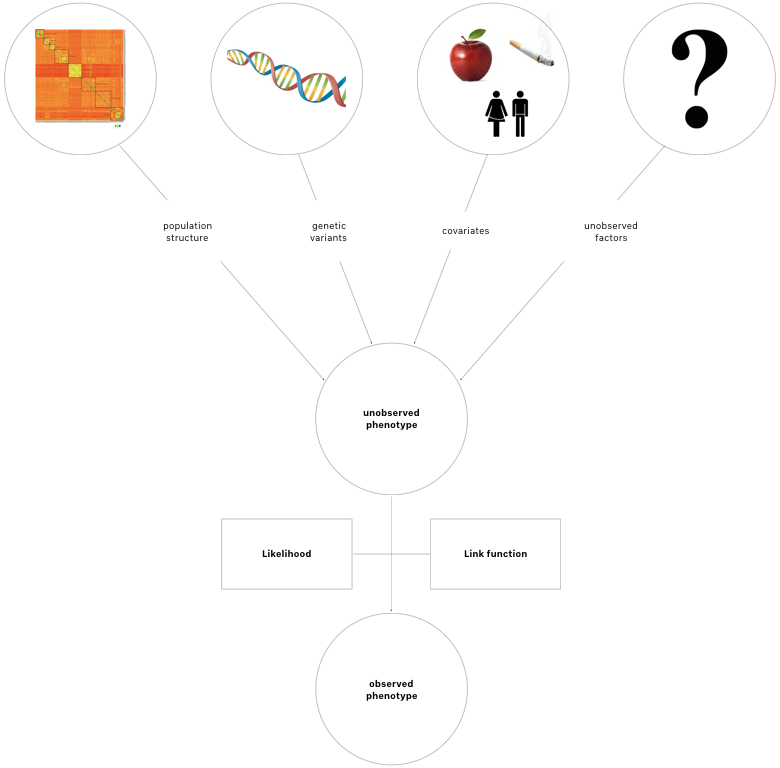
\includegraphics[width=0.5\textwidth]{images/friendly-model.png}
\end{figure}

Therefore the user is free to choose the distribution that represent the
observed process, as long as it can be completly defined by specifying its mean.
